\noindent
\subsection{Frequency domain analysis}
\label{spectrogram}
 


We perform the frequency domain analysis of 
the time series extracted from the temporal network
%We can convert a time series from its time domain to its frequency domain using Discrete Fourier Transform (DFT). However, instead of taking the discrete fourier transform of the whole series we 
by conducting
  a spectrogram analysis of the data. Spectrogram analysis is a short time fourier transform 
where we divide the whole time series into several equal sized windows and apply discrete fourier transform on this windowed data.
The main advantages of using spectrogram analysis are
 (a). we do not lose the time information,
 (b). we are able to obtain a view of the local frequency spectrum.
Also note that the spectrogram analysis allows us to identify as well as quantify the fluctuations in the data which is difficult to identify 
from the corresponding time series. 
A high concentration of low frequency components would indicate lower fluctuations in the data; in contrast no such concentration of low frequency components 
would indicate higher fluctuations and irregularities in the data.
%These fluctuations have a direct relation to our prediction framework as lower the fluctuations in data higher is the prediction accuracy and vice versa.

\begin{figure}
 \begin{center}
 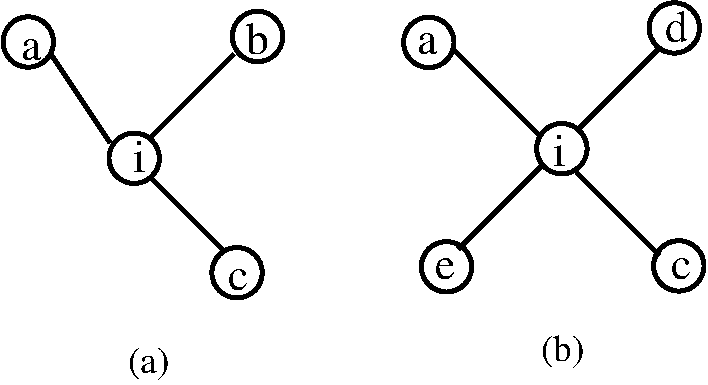
\includegraphics[width=0.45\columnwidth, angle=0]{./texfiles/Chapter_1/fig/jaccard-eps-converted-to.pdf}
 \caption{\label{fig2}(a) and (b) denote the status of node $i$ at time $t$ and $t+k$ respectively. $NBR(i)_{t}=\{a,b,c\}$ and $NBR(i)_{t+k}=\{a,d,c,e\}$ 
 $Correlation(i)_{k}$={\large$\frac{NBR(i)_{t}\bigcap NBR(i)_{t+k}}{NBR(i)_{t}\bigcup NBR(i)_{t+k}}$}={\large$\frac{2}{5}$} where $NBR(i)_{t}\rightarrow$ the set of neighbors of $i$ at time $t$}
  \end{center}
 \end{figure}

We construct the spectrogram and segregate the power spectral density (PSD measured in Watts/Hz) based on the frequency into three bins. In bin 1 we calculate the mean PSD 
corresponding to the frequencies $<$ 5 Hz, in bin 2 we calculate the PSD corresponding to frequencies between 5 and 15 Hz and bin 3 consists of the 
mean PSD value corresponding to frequencies $>$ 15 Hz. We call them LPSD, MPSD and HPSD respectively.
So a higher value of mean PSD corresponding to bin 1 (LPSD) would indicate lower fluctuations in data. 
In figures ~\ref{fig_all_dataset}(B), (D), (E) and ~\ref{fig_all_dataset_1}(B), (D) we plot the PSD corresponding to the three bins across all the properties for all the datasets. We 
observe that the lower frequencies dominate to a higher extent in case of the properties like number of active nodes, number of active edges, modularity 
but to a much lower extent in case of betweenness centrality, closeness centrality and clustering coefficient.  
In fact, as we shall show later, the prediction accuracy of a property can be enhanced through spectrogram analysis.
%this could be a good indicator of prediction accuracy of a property.
% But for the human face-to-face networks the PSD values 
% are much higher than in case networks of human contact through social media. This indicates that the time series corresponding to human face-to-face 
% network are more consistent and hence correlated than the network representing human contact through social media.



% Thus both the time domain analysis and the frquency domain analysis indicate that the evolution dynamics of human contact network through physical proximity (face-to-face) 
% and through social media differ significantly and it is almost impossible to obtain a generic growth model for these networks.
% In figure~\ref{fig10} we plot the spectrograms for number of active nodes and betweenness centrality for both INFOCOM 2006 and SIGCOMM 2009 datasets.
% Spectrogram analysis also requires the size of the series to be in the power of 2 or else it pads the rest of the time points until the closest power of 2
% with zeros. Therefore, we select 1024 time steps from 51 to 1074 in case of INFOCOM 2006 dataset and 43 to 1067 in case of SIGCOMM 2009 dataset.
% 
% Since we are not losing the time information as well as getting the local information, we use spectrograms in two ways-
% \begin{itemize}
%  \item From the spectrogram of the whole series we can determine whether this property of the network can be predicted with minimum error.
%  \item Using the local information we can determine whether a prediction at a certain time point would be erroneous or not before applying our prediction technique.
% \end{itemize}

% We have previously seen that for the property number of active nodes, we get the best prediction results and for betweenness centrality we obtain worse results.
% Here we check whether we can distinguish these two properties using the spectrogram of the whole time series. 
% In the figure ~\ref{fig10}(a) (spectrogram for number of active nodes), we find that throughout all the windows the frequency spectrum 
% is highly dominated by the low frequencies within range 0-3 Hz. In contrast if we look at the figure of 13(b) (spectrogram for betweenness centrality), we find a 
% very different behavior. In most of the windows the frequency spectrum consists of a number of frequencies and from the color bar it can be seen that 
% none of them dominates. These observations also hold for the other properties as well. Thus, we may conclude that the spectrogram response determines
% the goodness of our prediction. 
% If the frequency spectrum is distributed we conclude that the prediction may not be accurate for this time step. While if the 
% spectrogram is concentrated only to a small range of low frequencies, the predictions should be far better.
% 
% We now outline how to use spectrograms to make our predictions better. When predicting the value at any time step, before applying the prediction technique 
% we plot the spectrogram of the previous 128 time points. By analyzing this spectrogram, we determine whether our framework, on application would provide 
% significantly accurate predictions. For our analysis we considered the respective spectrograms for low prediction error time points and high prediction error 
% time points. 
% 
% 
%  In figure ~\ref{fig11} we show spectrograms of two such time points: one with prediction error around 1\% and the other with a prediction error of 98\%. 
%  It can be observed that in the former case the frequency spectrum is dominated with low frequencies while the other frequencies have negligible influence 
%  on the spectrogram. On the other hand for the latter case the spectrum is influenced by a large set of frequencies although very loosely. 
%  Note that these results are representative and 
%  similar observations were encountered for other points as well. Thus while predicting the value of the series at any time point we conduct a spectrogram  
%  analysis and conclude whether our framework would produce significantly accurate results.


\medskip
